\chapter{Architecture et implémentation}
\label{chapitre:architecture}

Ce chapitre relie la méthodologie au code exécuté. Le noyau HYPO, son évaluation principale,
l'extension bidirectionnelle et l'interface sont séparés afin qu'une modification de
présentation ne change pas silencieusement les résultats
\citep{sculley2015hidden,amershi2019software,breck2017ml}.

\section{Organisation du logiciel}

Le Tableau~\ref{tab:modules} récapitule les modules qui produisent les sorties du mémoire.

\begin{table}[H]
  \centering
  \caption{Modules qui produisent les sorties du mémoire.}
  \label{tab:modules}
  \small
  \begin{tabular}{p{0.35\textwidth}p{0.55\textwidth}}
    \toprule
    Module & Responsabilité \\
    \midrule
    \texttt{core/io.py} & Chargement, noms de colonnes et types temporels. \\
    \texttt{core/features.py} & Agrégation à quinze minutes, couverture et variables dérivées. \\
    \texttt{core/early\_warning.py} & Branche HYPO, période de référence, score, CUSUM et persistance. \\
    \texttt{core/hybrid\_warning.py} & Branche INSTABILITÉ et cinq règles de fusion. \\
    \texttt{core/pipeline.py} & Orchestration vache par vache et sortie troupeau. \\
    \texttt{core/model\_if.py} & Isolation Forest conservé comme comparateur visuel. \\
    Campagne HYPO & Validation principale après la période de référence. \\
    Ablation HYPO & Comparaison contre IF, LOF et le comparateur pédométrique. \\
    Sensibilité HYPO & Analyse OFAT des paramètres sans sélection de nouvelle configuration. \\
    \texttt{scripts/per\_cow\_calibration.py} & Test exploratoire d'un seuil individualisé. \\
    \texttt{scripts/detection\_}\\\texttt{background\_curve.py}
      & Courbe descriptive détection--charge. \\
    Profils de l'extension bidirectionnelle & Douze scénarios synthétiques et contrôles. \\
    Campagne de l'extension bidirectionnelle & Injections après la période de référence et métriques attribuables. \\
    Sensibilité de la fusion & Comparaison des fusions et sensibilité technique. \\
    Analyse IceTag--SLS synchronisée & Cohorte et mesures SLS. \\
    \texttt{app.py}, \texttt{ui/} & Interface Streamlit de priorisation. \\
    \texttt{tests/} & Tests unitaires, invariants et non-régression. \\
    \bottomrule
  \end{tabular}
\end{table}

Les fichiers du dossier \texttt{scripts/} servent aux tâches reproductibles de soutien:
génération des figures, orchestration de la validation HYPO et mesure de performance. Ils
n'introduisent pas une logique de détection parallèle. Le script
\texttt{run\_hypo\_module\_validation.py} produit les artefacts de la campagne principale et
de l'ablation; \texttt{benchmark\_performance.py} chronomètre la chaîne de traitement complète; et
un script dédié produit les figures de l'extension. Les scripts
\path{per_cow_calibration.py} et \path{detection_background_curve.py} réutilisent la
campagne HYPO sans introduire de nouvelle logique d'alerte. La
Figure~\ref{fig:architecture_modules} schématise cette organisation.

\begin{figure}[H]
  \centering
  \resizebox{0.98\textwidth}{!}{%
  \begin{tikzpicture}[
    box/.style={rectangle, draw=black!60, rounded corners=2pt, minimum height=0.9cm,
      text width=3.2cm, align=center, font=\small, inner sep=7pt},
    arrow/.style={-{Stealth[length=2.3mm]}, thick, black!65}]
    \node[box, fill=profgray!10] (data) {CSV IceQube\\par vache};
    \node[box, fill=ifblue!10, right=0.7cm of data] (features) {Intervalles\\et couverture};
    \node[box, fill=rulegreen!12, right=0.8cm of features, yshift=0.8cm] (hypo) {Branche HYPO\\12 h / 6 h};
    \node[box, fill=loforange!12, right=0.8cm of features, yshift=-0.8cm] (inst) {Branche INSTABILITÉ\\3 h / 2 h};
    \node[box, fill=ifblue!8, right=1.0cm of hypo, yshift=-0.8cm] (fusion) {Fusion\\hiérarchique};
    \node[box, fill=profgray!8, right=0.8cm of fusion, yshift=0.7cm] (action) {Notification de\\vérification};
    \node[box, fill=profgray!8, right=0.8cm of fusion, yshift=-0.7cm] (surv) {Surveillance\\d'instabilité};
    \draw[arrow] (data) -- (features);
    \draw[arrow] (features.east) -- ++(0.35,0) |- (hypo.west);
    \draw[arrow] (features.east) -- ++(0.35,0) |- (inst.west);
    \draw[arrow] (hypo) -- (fusion); \draw[arrow] (inst) -- (fusion);
    \draw[arrow] (fusion) -- (action); \draw[arrow] (fusion) -- (surv);
  \end{tikzpicture}}
  \caption{Architecture du système.}
  \label{fig:architecture_modules}
\end{figure}

\section{Flux de traitement}

Pour une vache, \texttt{run\_pipeline\_one\_cow} effectue les opérations suivantes:
\begin{enumerate}
  \item normaliser les mesures et construire les intervalles;
  \item matérialiser la séparation entre la période de référence et la période future;
  \item exécuter le comparateur Isolation Forest;
  \item calculer la branche HYPO;
  \item calculer la branche INSTABILITÉ;
  \item appliquer la fusion choisie et espacer les notifications;
  \item retourner les scores, épisodes, départs, notifications, types et priorités.
\end{enumerate}
La chaîne appliquée au troupeau répète ce traitement sans partager de période de référence
entre les vaches.

\section{Implémentation des deux persistances}

La persistance n'est pas appliquée après une fusion brute. Chaque branche construit d'abord
ses propres candidats, son propre CUSUM et son propre épisode. Cette décision évite qu'une
instabilité courte doive durer six heures pour être reconnue ou qu'une baisse lente soit
déclenchée par deux heures de fluctuation. La fusion reçoit donc deux séries d'épisodes déjà
stabilisées.

Dans la branche HYPO, une fenêtre glissante de six heures doit contenir au moins 45\,\% de
candidats et le CUSUM doit franchir 1,20. Dans la branche INSTABILITÉ, la proportion minimale
est de 50\,\% sur deux heures et le CUSUM doit franchir 0,70. Ces règles sont déterministes et
testées séparément.

\section{Fusion hiérarchique}

La fusion hiérarchique est volontairement asymétrique. Une instabilité seule indique une
situation à surveiller, mais ne déclenche pas automatiquement une vérification prioritaire.
Une hypoactivité produit une notification de vérification. La priorité augmente lorsque les deux
branches convergent ou lorsqu'un départ HYPO est précédé d'un départ INSTABILITÉ dans la
fenêtre de 72 heures. Cette architecture empêche un simple pic de \textit{Motion Index} de
devenir une notification de vérification.

L'algorithme~\ref{alg:fusion} formalise cette logique de fusion pour une vache donnée.

\begin{figure}[H]
\centering
\fbox{\parbox{0.92\textwidth}{\raggedright
\textbf{Algorithme:} Fusion hiérarchique des branches HYPO et INSTABILITÉ (par vache)
\vspace{0.3em}\hrule\vspace{0.5em}
\textbf{Entrée:} intervalles $X$ d'une vache, période de référence individuelle, paramètres $\theta$\\
\textbf{Sortie:} type d'alerte, priorité et notifications (alerte à vérifier, non diagnostique)

\begin{enumerate}[leftmargin=1.5em]
\item \textit{Détection des deux branches:}\\
    $\mathrm{hypo} \leftarrow \textsc{DétecterHypo}(X,\ \text{référence},\ \text{persistance} = 6\,\text{h})$
    \hspace{0.5em}(baisse d'activité persistante)\\
    $\mathrm{instab} \leftarrow \textsc{DétecterInstabilité}(X,\ \text{référence},\ \text{persistance} = 2\,\text{h})$
    \hspace{0.5em}(mouvement disproportionné aux pas)

\item \textit{Fusion par priorité décroissante:}\\
    Si $\mathrm{hypo}$ et $\mathrm{instab}$ récente ($\leq 72\,\text{h}$)\,:\quad
    priorité $\leftarrow 3$,\ \ type $\leftarrow$ \texttt{SEQUENCE}\\
    Sinon si $\mathrm{hypo}$ et $\mathrm{instab}$\,:\quad
    priorité $\leftarrow 3$,\ \ type $\leftarrow$ \texttt{MIXTE}\\
    Sinon si $\mathrm{hypo}$\,:\quad
    priorité $\leftarrow 2$,\ \ type $\leftarrow$ \texttt{HYPO}\\
    Sinon si $\mathrm{instab}$\,:\quad
    priorité $\leftarrow 1$,\ \ type $\leftarrow$ \texttt{SURVEILLANCE}
    \hspace{0.5em}(à surveiller, sans vérification prioritaire)

\item \textit{Notification:}\\
    Émettre une notification seulement si priorité $\geq 2$\\
    Respecter un délai réfractaire de fusion de $12\,\text{h}$ entre notifications
\end{enumerate}
}}
\caption{Pseudocode de la fusion hiérarchique des deux branches.}
\label{alg:fusion}
\end{figure}

\section{Comparateurs Isolation Forest et Local Outlier Factor}
\label{sec:comparateurs}

Deux détecteurs d'anomalies non supervisés sont conservés comme points de comparaison. Ils
ne produisent pas la notification principale~: ils situent le détecteur temporel par rapport
à des familles d'algorithmes répandues et fournissent des points de comparaison reproductibles.

\subsection{Isolation Forest}

Isolation Forest isole les observations rares en construisant des arbres de partition
aléatoire~: un point anormal, plus facile à séparer du reste, présente une profondeur
moyenne d'isolation plus faible \citep{liu2008isolation}. Les variables dérivées sont
d'abord mises à l'échelle par un \texttt{RobustScaler} (intervalle inter-quantile
10--90), qui résiste aux distributions fortement asymétriques des signaux d'activité. Le
modèle est ajusté sur la période de référence de chaque vache, puis appliqué à l'ensemble de sa
série, de sorte qu'il décrive l'écart d'un intervalle par rapport au comportement
individuel appris. Les hyperparamètres figés sont rassemblés au
Tableau~\ref{tab:if_hyperparams}.

\begin{table}[H]
  \centering
  \caption{Hyperparamètres figés d'Isolation Forest (comparateur).}
  \label{tab:if_hyperparams}
  \small
  \begin{tabular}{p{0.30\textwidth}p{0.22\textwidth}p{0.36\textwidth}}
    \toprule
    Hyperparamètre & Valeur & Rôle \\
    \midrule
    Nombre d'arbres & 800 & Stabilité du score d'isolation \\
    Variables par arbre & 0,80 & Décorrélation des arbres \\
    Échantillonnage & \textit{bootstrap} & Diversité des sous-ensembles \\
    Contamination & 0,06 & Fraction supposée d'anomalies \\
    Graine aléatoire & 42 & Reproductibilité exacte \\
    Mise à l'échelle & RobustScaler 10--90 & Robustesse à l'asymétrie \\
    Ajustement & période de référence & Référence propre à chaque vache \\
    \bottomrule
  \end{tabular}
\end{table}

Les sorties \texttt{if\_score} et \texttt{if\_anomaly\_point}, ainsi que des colonnes de
compatibilité \texttt{pred\_lameness\_*}, restent disponibles. Elles alimentent l'ablation
du Chapitre~\ref{chapitre:validation} et l'affichage, sans jamais définir la conclusion. Par
construction, Isolation Forest repère un écart \emph{ponctuel} dans n'importe quelle
direction~; il ne modélise ni la référence horaire individuelle, ni la \emph{direction}, ni
la \emph{persistance} d'une dégradation, qui sont précisément les propriétés recherchées par
la branche HYPO.

\subsection{Local Outlier Factor}

Local Outlier Factor compare la densité locale d'un point à celle de ses voisins~: une
densité nettement plus faible que le voisinage signale une anomalie locale
\citep{breunig2000lof}. Il est exécuté en mode nouveauté dans le module d'ablation,
avec les mêmes indices d'entraînement et la même normalisation robuste que la comparaison
Isolation Forest, afin que l'écart mesuré reflète l'algorithme et non un changement de
protocole. Sa complexité quadratique dans le cas général le rend moins apte au passage à
l'échelle, mais il peut capter des structures locales que les méthodes globales manquent.
Le Tableau~\ref{tab:if_vs_lof} du Chapitre~\ref{chapitre:contexte} résume leurs propriétés
respectives.

\section{Implémentation des validations}

Le module de campagne HYPO sélectionne les vaches admissibles, exécute une
référence propre et injecte les quatre profils de la campagne HYPO. Le module
d'ablation réutilise les mêmes fenêtres pour les cinq variantes. Le
module d'extension bidirectionnelle étend ensuite le protocole aux douze scénarios
bidirectionnels. Le harnais garantit trois propriétés~: un placement reproductible des
perturbations, une attribution stricte de l'effet à l'injection, et le rejet de toute
campagne mal formée.

\subsection{Génération déterministe}

La graine d'une vache et d'un scénario est dérivée par SHA-256, indépendamment de la
variable d'environnement de hachage de Python~; deux exécutions produisent donc exactement
les mêmes injections. La position des profils est tournée entre les vaches pour ne pas
associer systématiquement une intensité à une période particulière. La fonction
d'injection renvoie une copie modifiée de la série et une table décrivant la fenêtre, les
changements cibles et la raison de conception, sans jamais altérer le fichier source.

\subsection{Exécution de référence et attribution}

Chaque vache est aussi exécutée \emph{sans} injection. Les nouveaux débuts de la série
injectée sont comparés aux débuts de cette référence avec une tolérance temporelle, et pour
la couverture comme pour l'IoU, le masque d'épisode de référence est soustrait intervalle
par intervalle du masque injecté. Cette étape est indispensable~: elle empêche de créditer
une injection lorsqu'une alerte identique aurait été produite par les données originales, et
c'est elle qui rend les métriques \emph{attribuables} (Section~\ref{sec:hypo}
du Chapitre~\ref{chapitre:methodologie}).

\subsection{Contrôles bloquants}

Avant tout calcul de résultat, le protocole vérifie l'unicité des identifiants d'événement,
leur non-chevauchement, leur placement strictement après la période de référence, la disponibilité des
signaux, la non-négativité des mesures, la conservation du temps postural total et l'absence
d'écriture dans le fichier source. Une campagne qui échoue à l'un de ces contrôles
n'alimente pas le manuscrit. La comparaison des fusions réutilise exactement les mêmes
vaches et les mêmes scénarios, de sorte que les écarts entre variantes ne tiennent qu'à la
règle de fusion.

\section{Évaluation du temps d'exécution}

L'évaluation reconstruit les variables, exécute le comparateur Isolation Forest, les règles
IF comparatives, HYPO, INSTABILITÉ et la fusion hiérarchique. Chaque étape est chronométrée avec
une horloge monotone. Cinq répétitions sont effectuées sur les 28 vaches et la concaténation
des sorties intervalle est incluse. Le résultat canonique est la médiane des cinq durées; les
valeurs minimale et maximale sont conservées pour rendre visible la variabilité de la machine.
Ce test documente la faisabilité du prototype sur l'ordinateur utilisé, non un temps garanti
en production.

\section{Technologies et dépendances}

Le Tableau~\ref{tab:technologies} présente les principales dépendances figées dans
\path{requirements.txt}. Les versions exactes servent à reconstruire l'environnement et à
garantir la reproductibilité numérique~; elles ne constituent pas un résultat scientifique.
Les comparateurs Isolation Forest et Local Outlier Factor proviennent de \texttt{scikit-learn}
\citep{sklearn_api}, les tests statistiques de \texttt{SciPy} \citep{virtanen2020scipy},
et l'interface de \texttt{Streamlit}; la manipulation des données et le calcul numérique
reposent sur \texttt{pandas} \citep{mckinney2010data} et \texttt{NumPy} \citep{harris2020array}.

\begin{table}[H]
  \centering
  \caption{Principales technologies de la version reproductible.}
  \label{tab:technologies}
  \small
  \begin{tabular}{lll}
    \toprule
    Composant & Version & Rôle principal \\
    \midrule
    Python & 3.10 ou ultérieur & Langage d'exécution \\
    pandas & 2.3.3 & Manipulation des données tabulaires \\
    NumPy & 2.3.5 & Calcul numérique \\
    scikit-learn & 1.7.2 & Comparateurs IF et LOF \\
    SciPy & 1.16.2 & Tests et statistiques descriptives \\
    statsmodels & 0.14.5 & Compléments statistiques \\
    Streamlit & 1.51.0 & Interface interactive \\
    Plotly & 6.3.0 & Tracés interactifs de l'interface \\
    pytest & 8.4.2 & Tests automatisés \\
    \bottomrule
  \end{tabular}
\end{table}

\section{Interface Streamlit}
\label{sec:interface_streamlit}

L'interface est un outil de lecture et de priorisation. Elle charge par défaut
\texttt{data/brut.csv} et accepte un CSV importé. La vue individuelle présente les signaux,
les épisodes et les notifications. La vue troupeau ordonne les animaux à vérifier, tandis
que la carte thermique permet une comparaison journalière. Isolation Forest reste présenté
comme comparateur; il ne constitue pas la notification principale.

\subsection{Niveaux de priorité et action associée}

L'interface traduit la sortie de fusion en trois niveaux de priorité qui orientent l'effort
de vérification, sans jamais affirmer un diagnostic (Tableau~\ref{tab:priorites}). Seules les
priorités~2 et~3 produisent une notification de vérification~; la priorité~1 reste un signal de
surveillance. Ce classement remplace une échelle de risque clinique~: il ordonne les animaux
à observer, il ne quantifie pas une probabilité de boiterie.

\begin{table}[H]
  \centering
  \caption{Niveaux de priorité de l'interface et action de vérification associée.}
  \label{tab:priorites}
  \small
  \begin{tabular}{cp{0.36\textwidth}p{0.38\textwidth}}
    \toprule
    Priorité & Condition & Action suggérée \\
    \midrule
    3 & Convergence HYPO + INSTABILITÉ, ou séquence instabilité$\rightarrow$hypoactivité &
    Vérification rapprochée, observation locomotrice \\
    2 & Hypoactivité persistante (HYPO) & Vérification à planifier \\
    1 & Instabilité isolée & Surveillance, sans alerte de vérification \\
    \bottomrule
  \end{tabular}
\end{table}

Les Figures~\ref{fig:streamlit_individual} à~\ref{fig:streamlit_heatmap} illustrent les
principales vues de l'interface. Les marqueurs affichés dans la vue individuelle signalent
une vérification à effectuer; ils ne confirment pas une boiterie. Les vues de troupeau
servent uniquement à ordonner les animaux et les journées à examiner.

\begin{figure}[H]
  \centering
  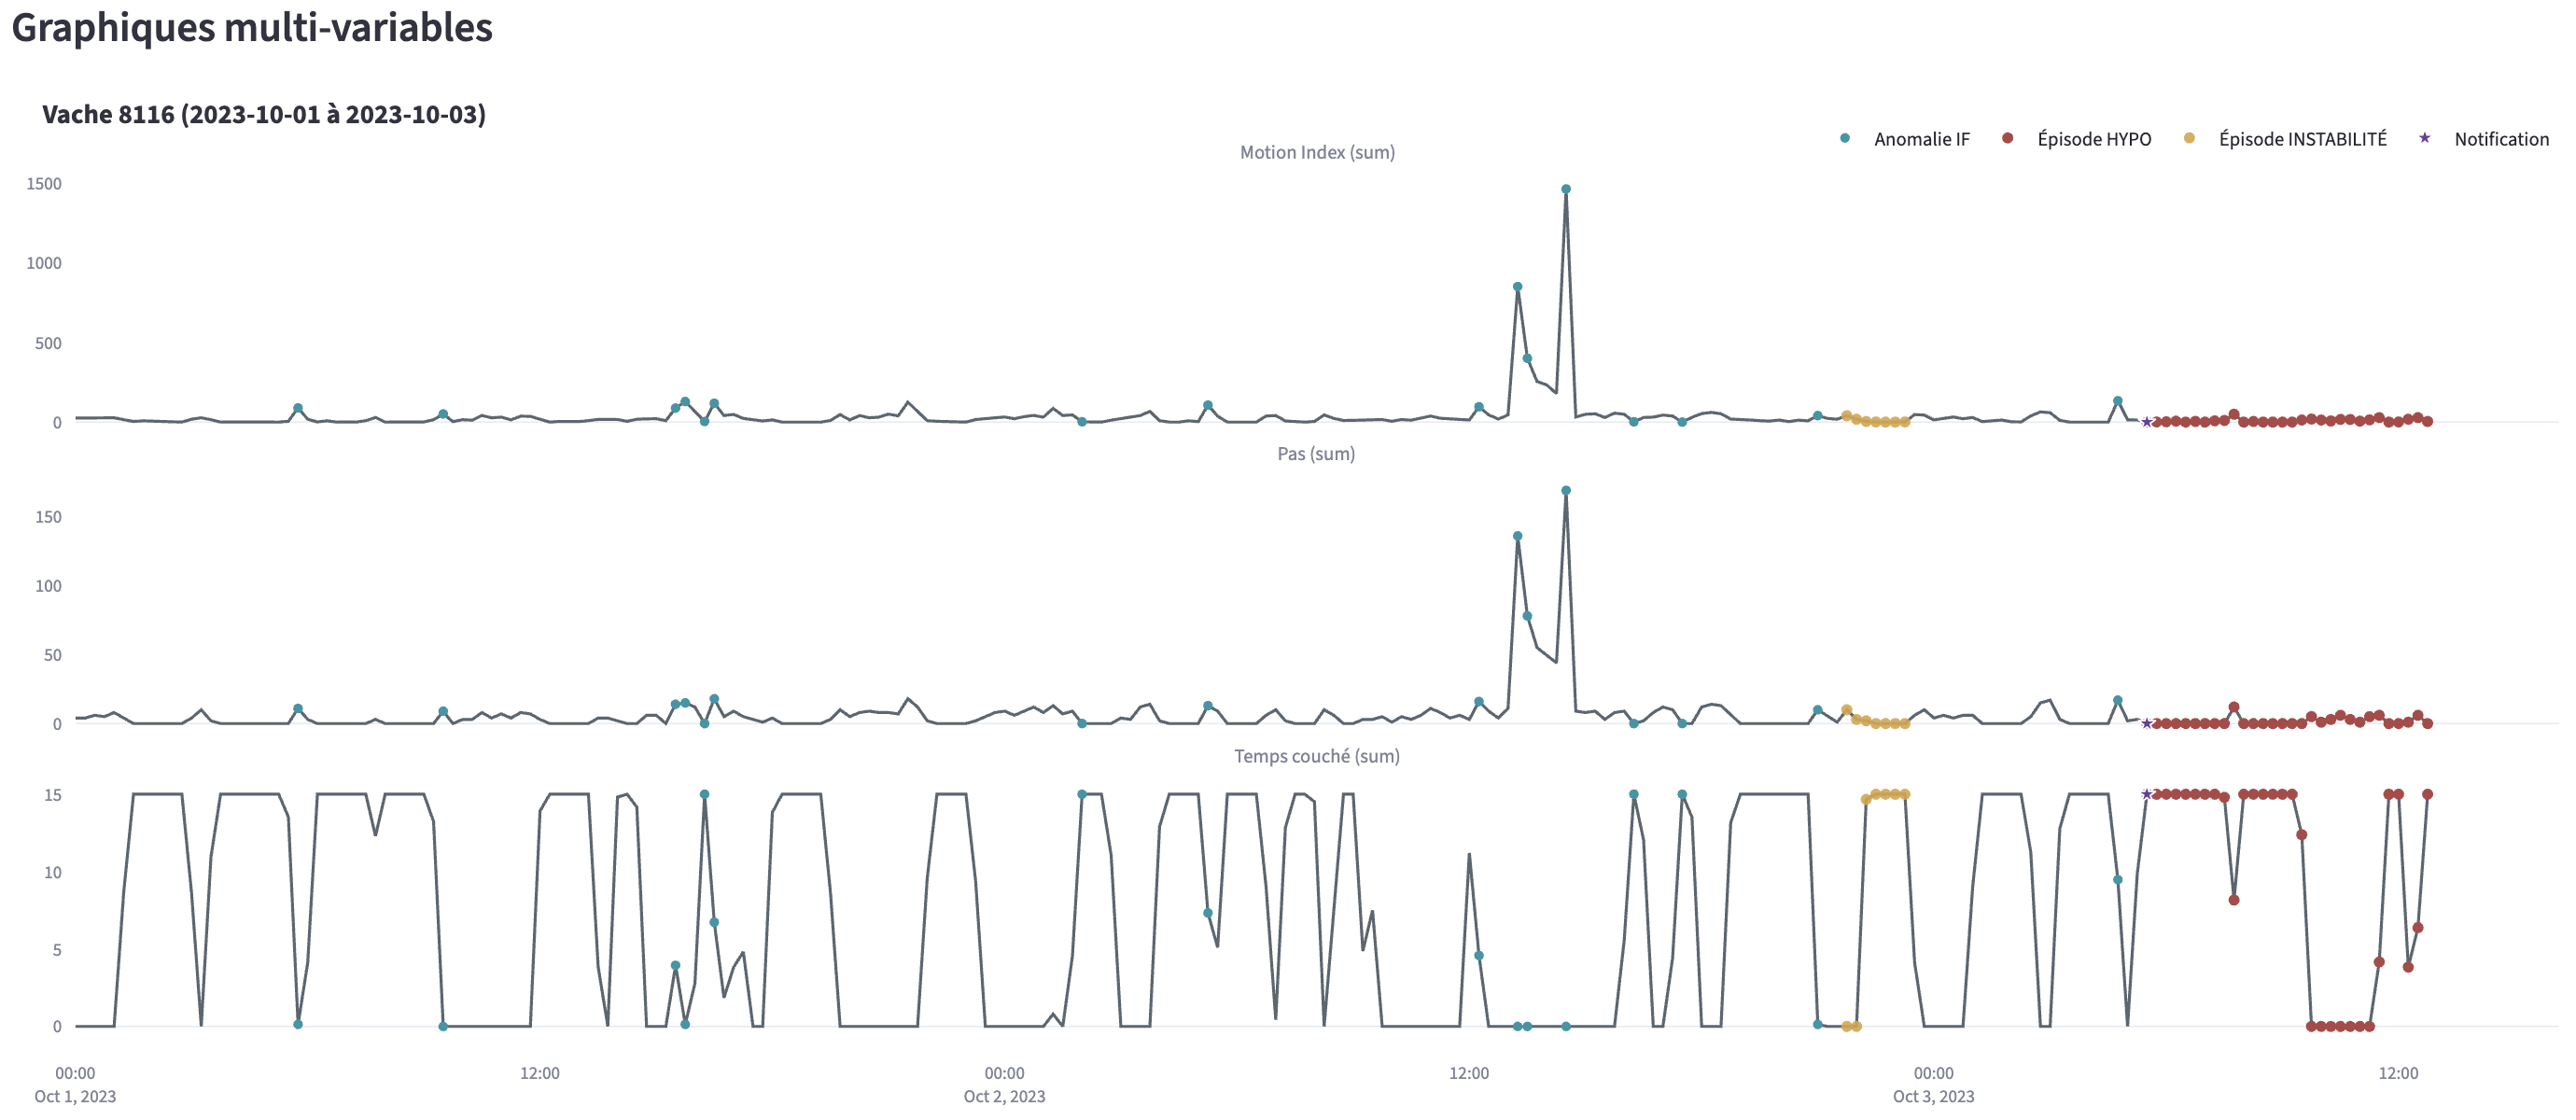
\includegraphics[width=0.98\textwidth]{figures/streamlit_individual.png}
  \caption{Analyse individuelle du tableau de bord.}
  \label{fig:streamlit_individual}
\end{figure}

\begin{figure}[H]
  \centering
  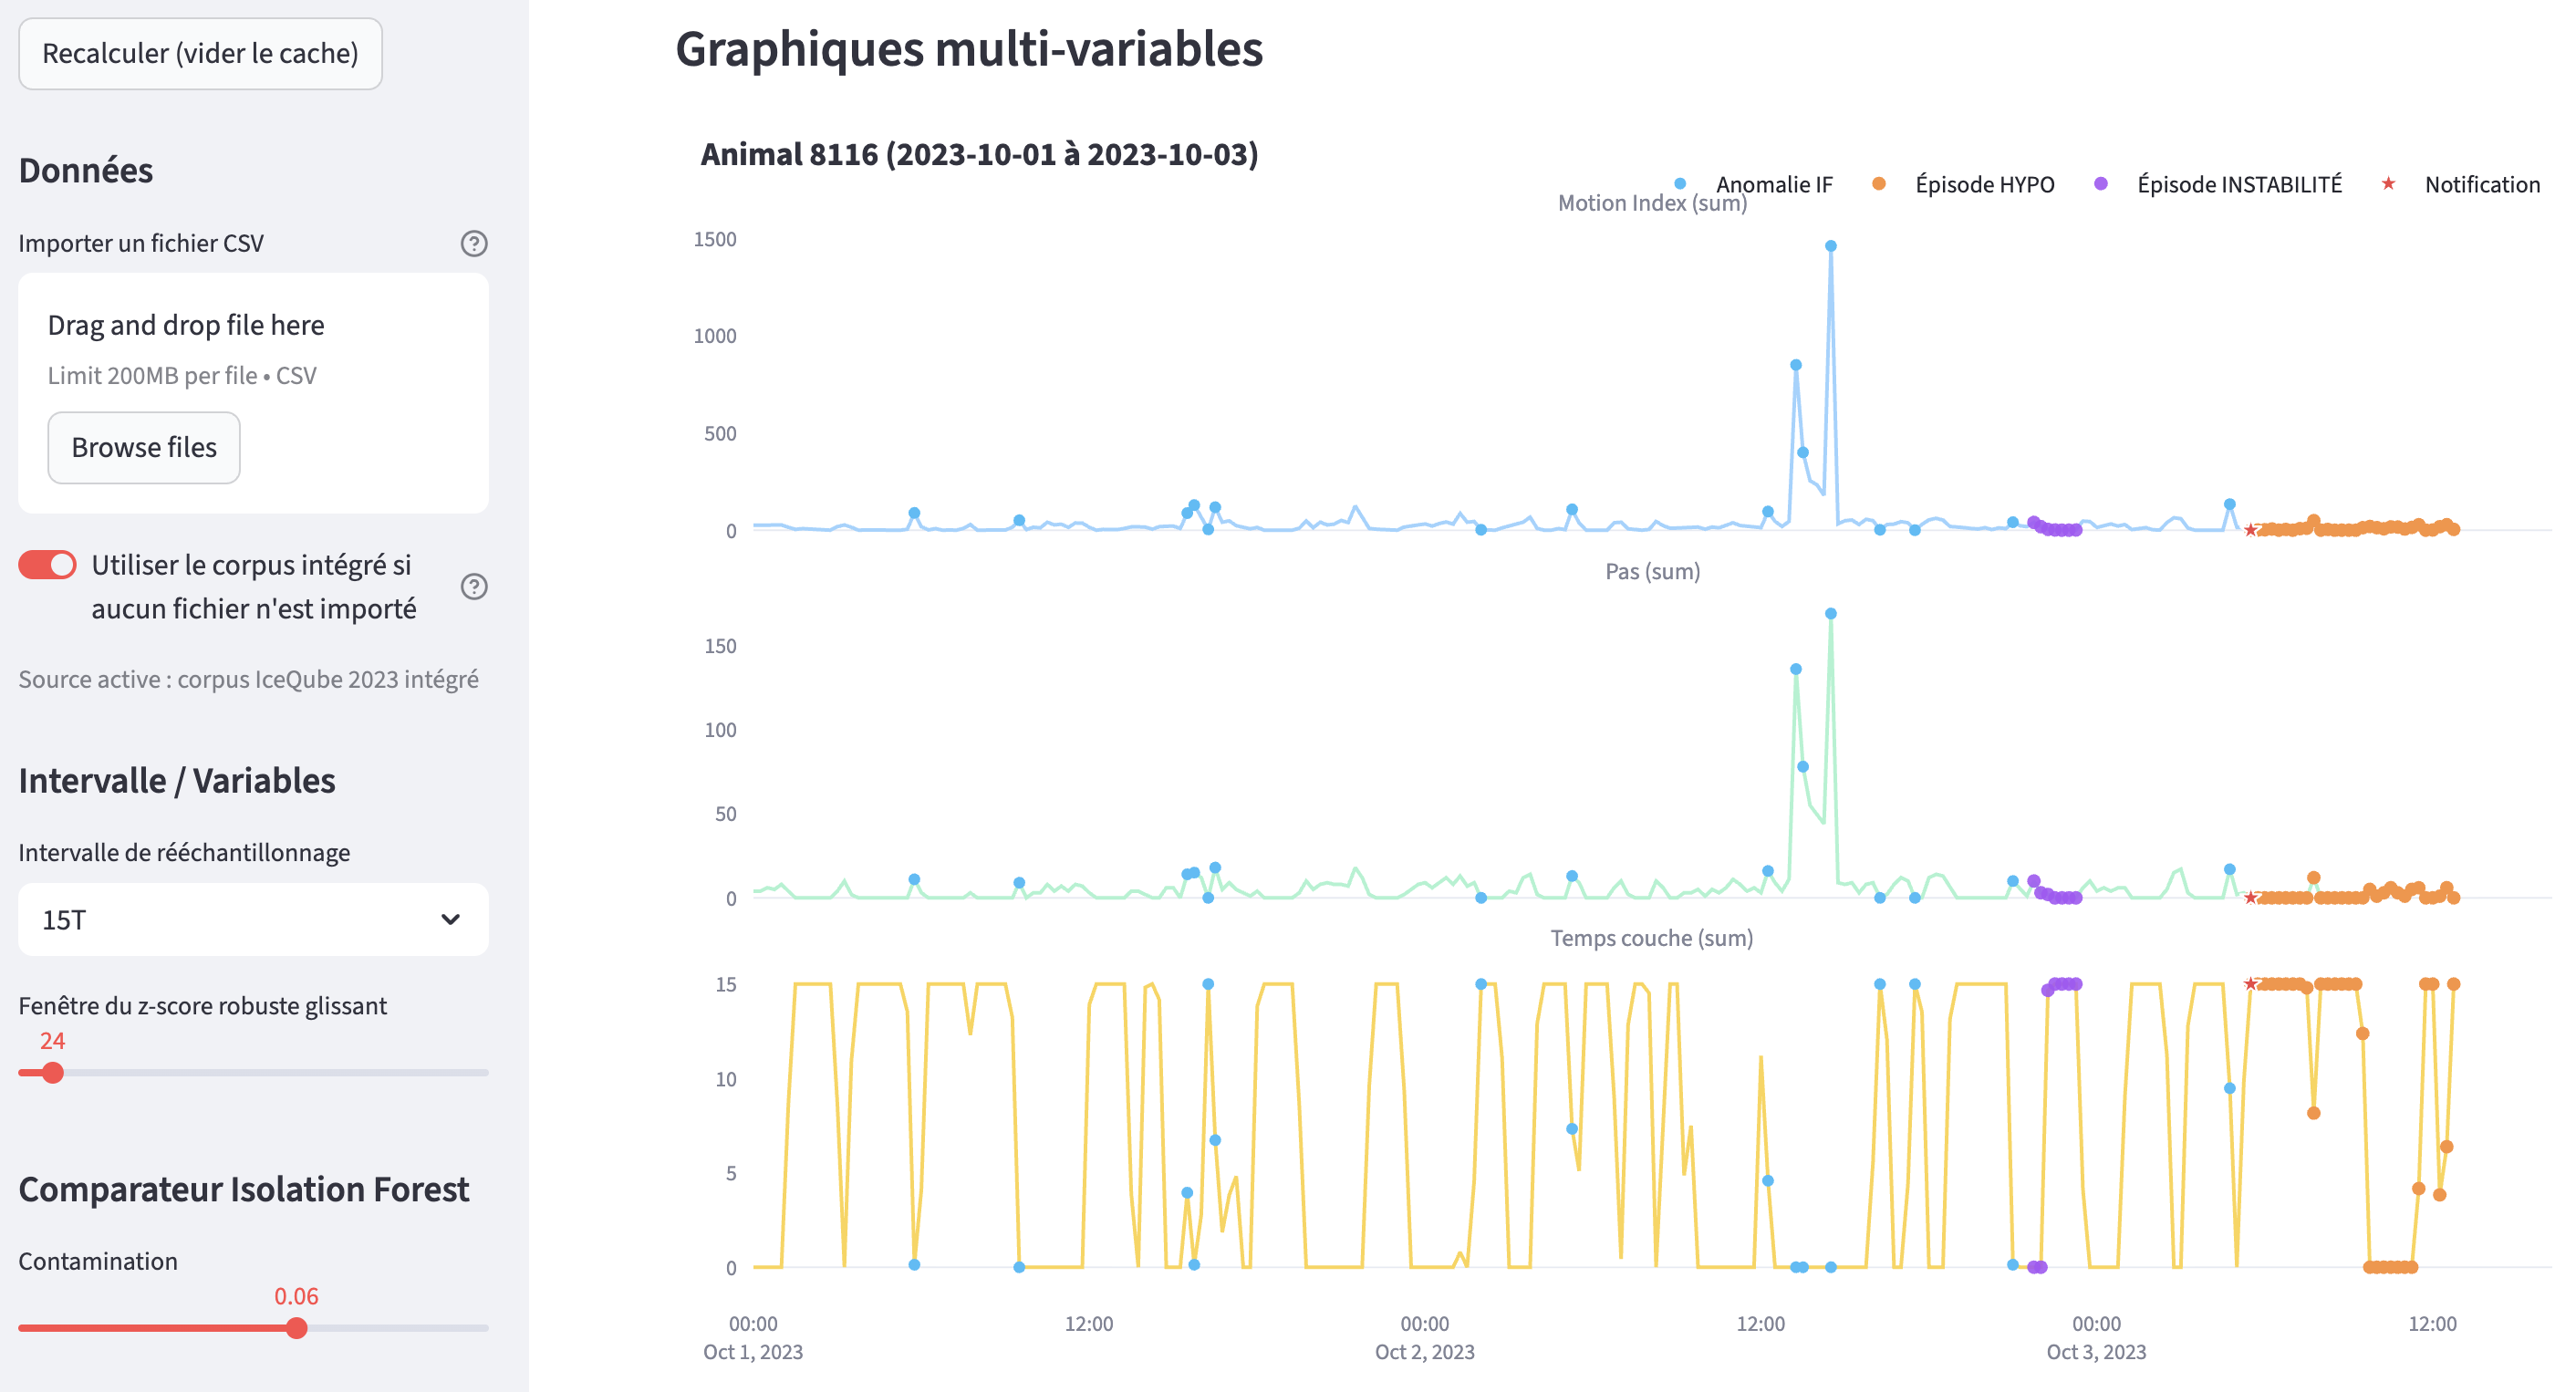
\includegraphics[width=0.98\textwidth]{figures/streamlit_individual_8116.png}
  \caption{Signaux de la vache 8116.}
  \label{fig:streamlit_individual_8116}
\end{figure}

\begin{figure}[H]
  \centering
  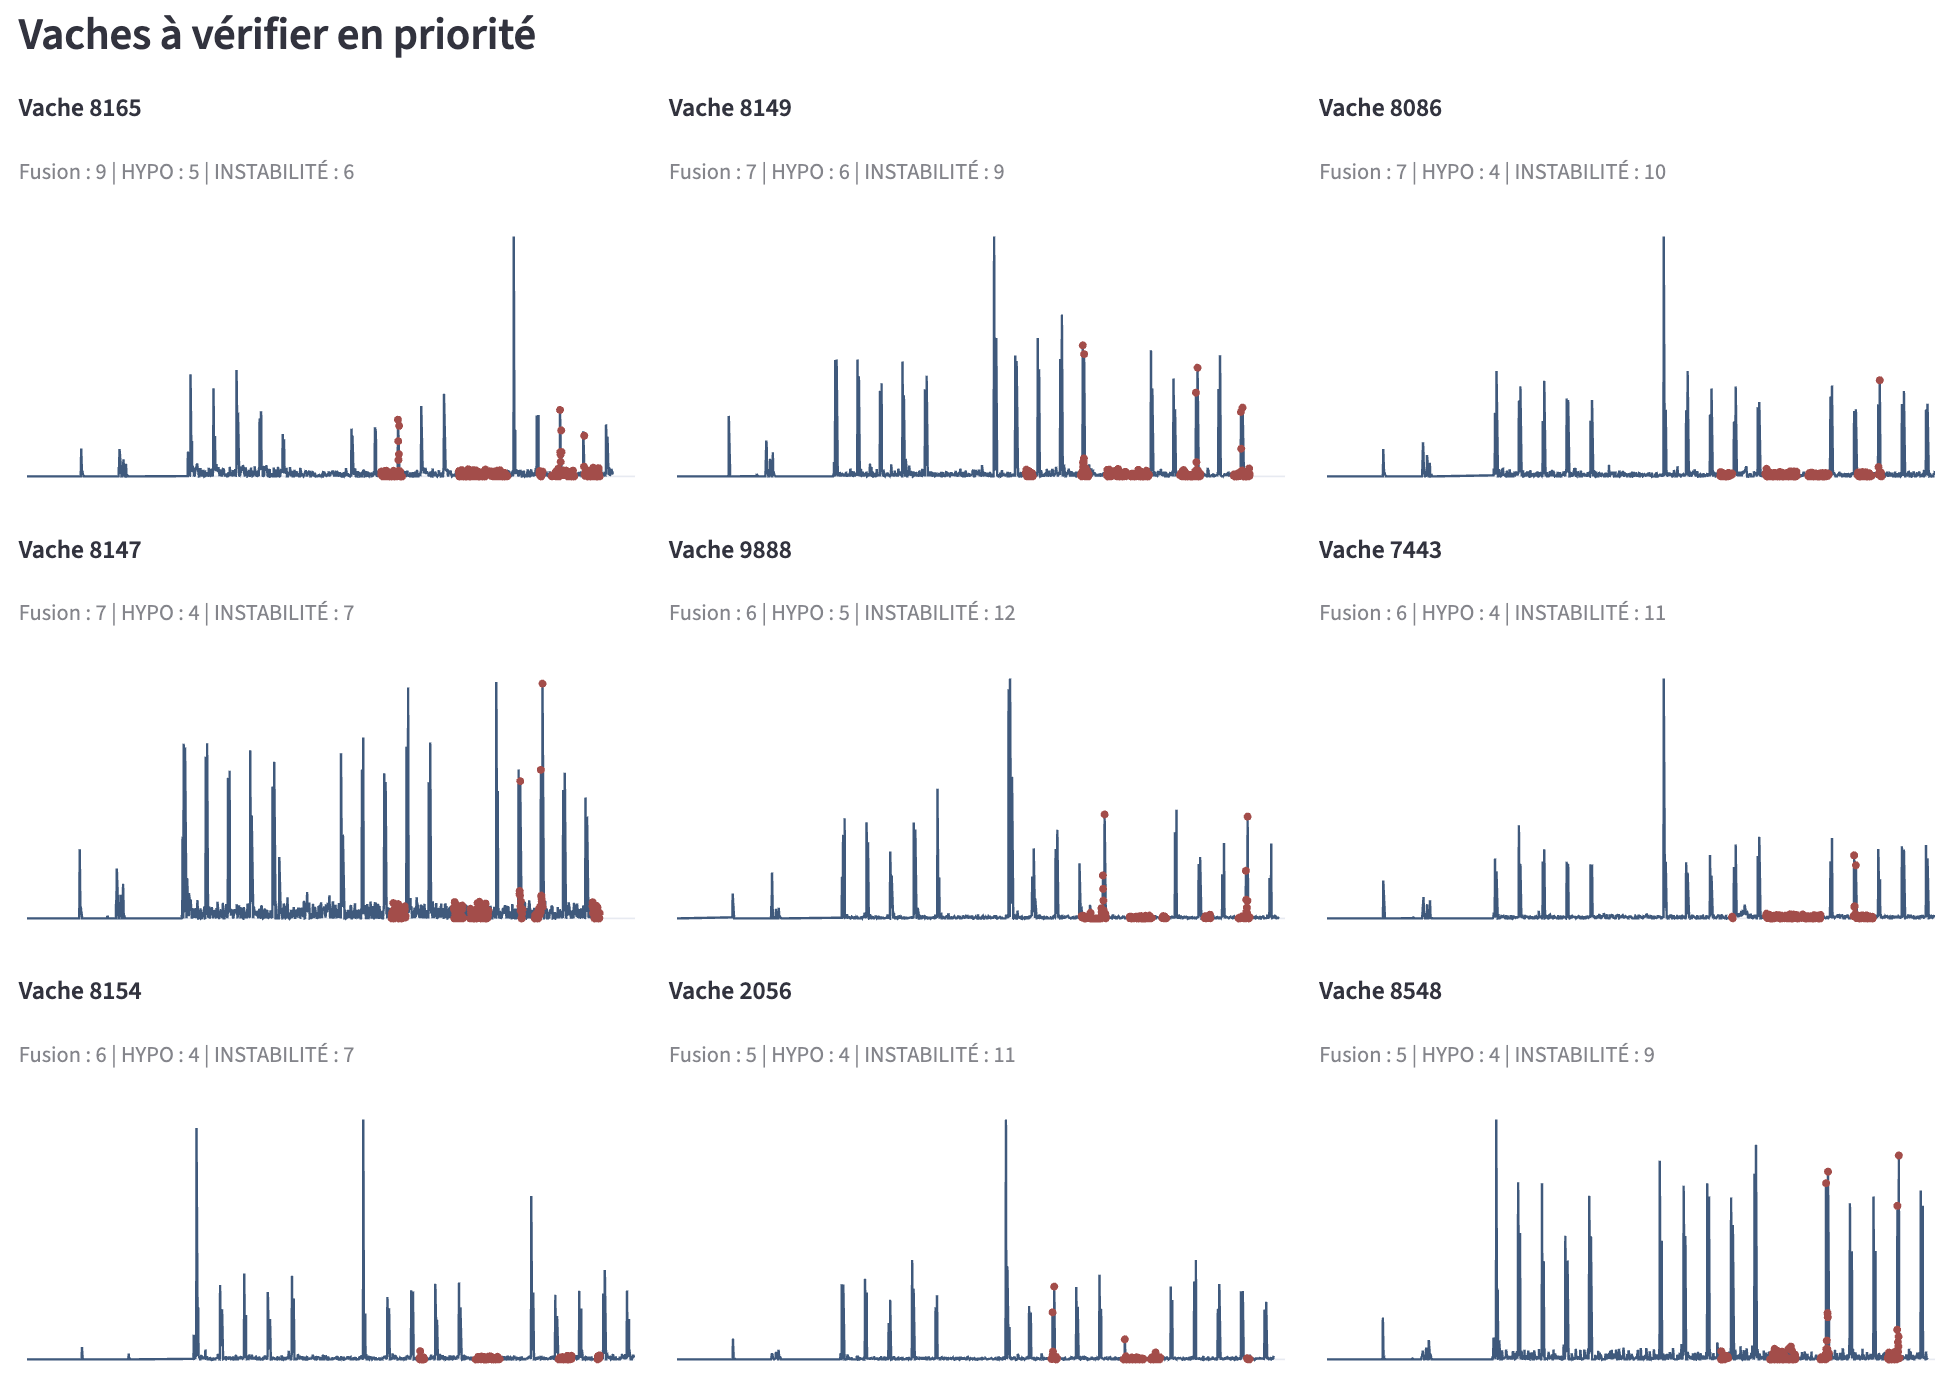
\includegraphics[width=0.98\textwidth]{figures/streamlit_priority_animals.png}
  \caption{Animaux à vérifier en priorité.}
  \label{fig:streamlit_priority_animals}
\end{figure}

\begin{figure}[H]
  \centering
  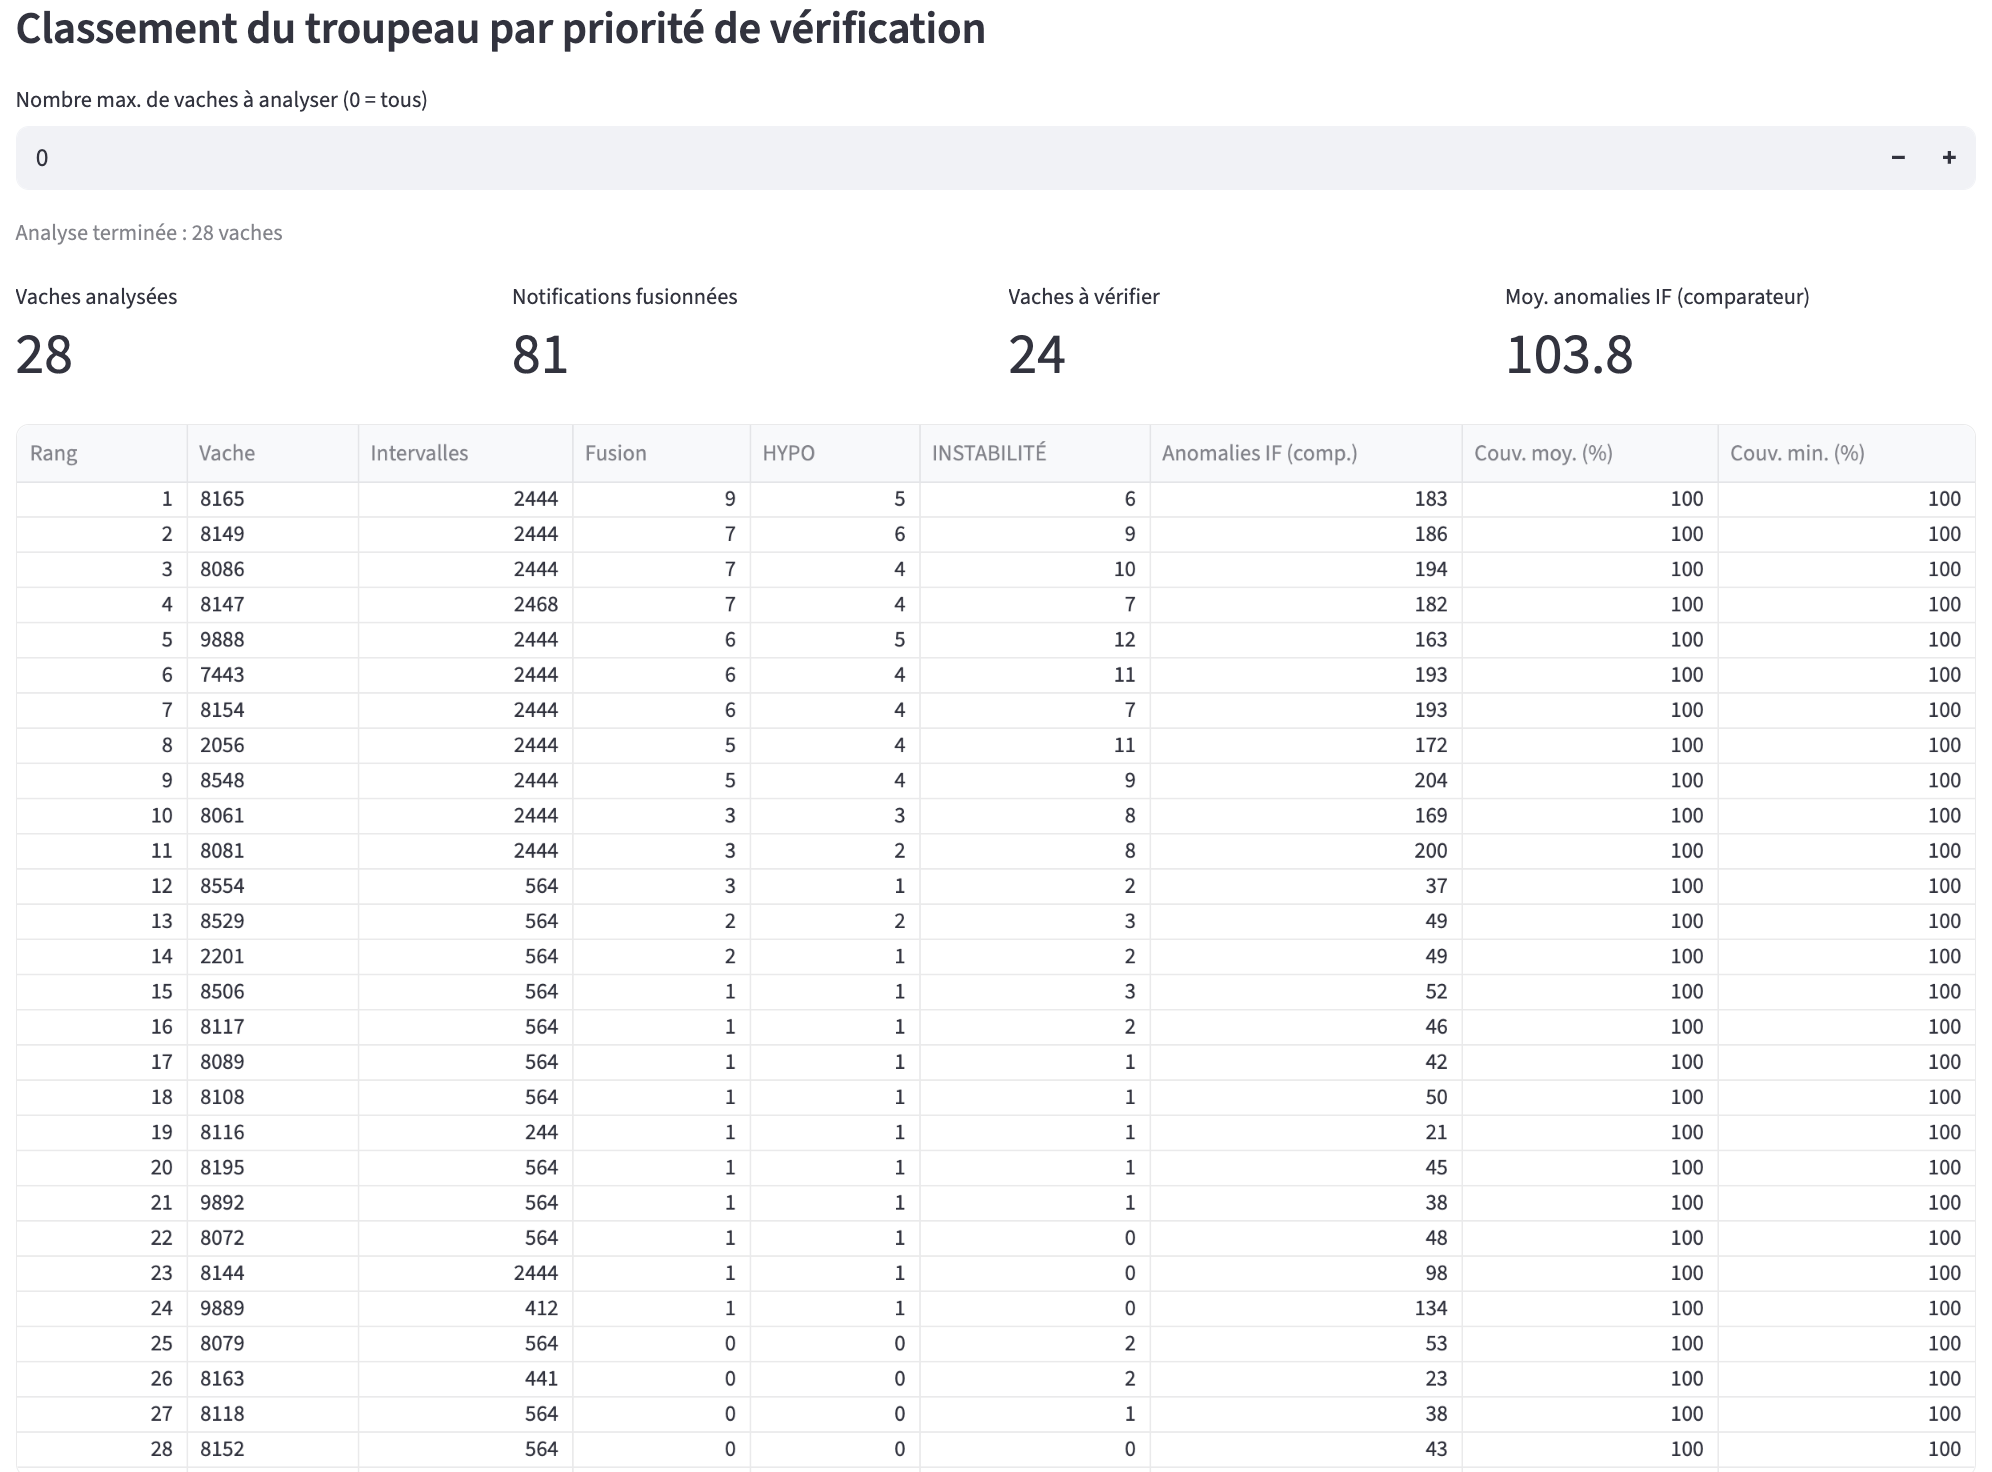
\includegraphics[width=0.98\textwidth]{figures/streamlit_herd_table.png}
  \caption{Classement du troupeau.}
  \label{fig:streamlit_herd_table}
\end{figure}

\begin{figure}[H]
  \centering
  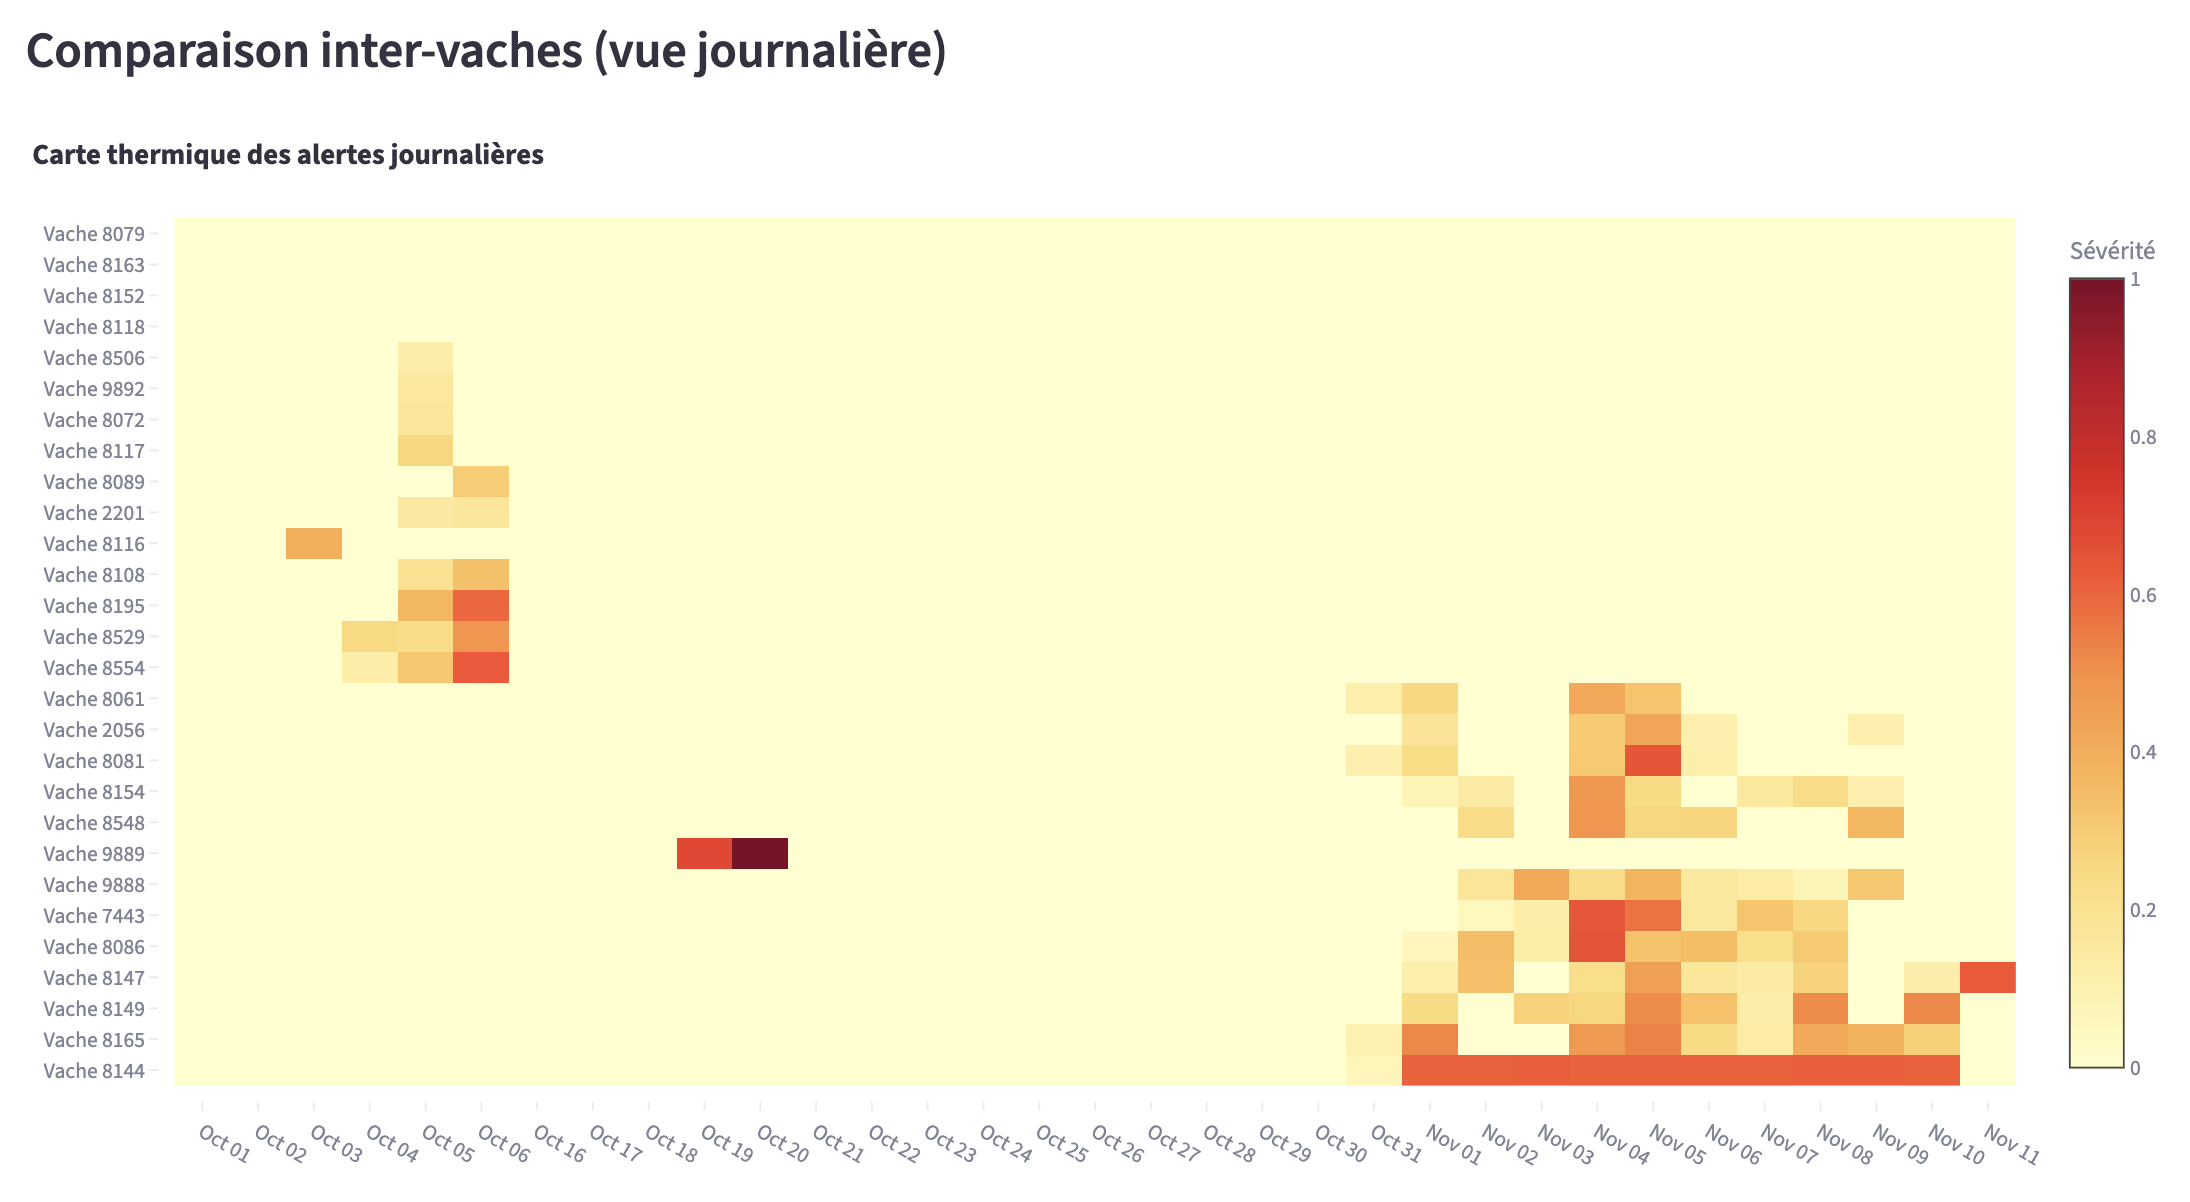
\includegraphics[width=0.98\textwidth]{figures/streamlit_heatmap_compact.png}
  \caption{Alertes journalières par animal.}
  \label{fig:streamlit_heatmap}
\end{figure}

\section{Tests et traçabilité}

La suite automatisée contient 98 tests. Elle couvre le chargement, les variables dérivées,
les deux détecteurs, les cinq fusions, les injections, les contrôles après la période de référence,
l'analyse de sensibilité, l'analyse SLS et le démarrage de Streamlit. Les résultats sont
écrits dans des fichiers tabulaires dont la provenance est explicite. Le succès des tests
atteste la cohérence logicielle, pas la validité clinique.

Chaque résultat suit un cycle de vie traçable~: une commande de reproduction exécute un
module de validation, qui écrit des fichiers CSV et JSON~; un manifeste SHA-256
fige ces sorties~; et un script dédié les transforme en figures du manuscrit. Aucun résultat
n'est saisi à la main. Une modification du code, des données ou des paramètres impose donc
une nouvelle exécution et un nouveau manifeste, de sorte que le PDF seul ne constitue jamais
la trace de référence de l'expérience. La Figure~\ref{fig:repro_chain} illustre cette chaîne.

\begin{figure}[H]
  \centering
  \resizebox{0.98\textwidth}{!}{%
  \begin{tikzpicture}[
    pbox/.style={rectangle, draw=black!60, rounded corners=2pt, align=center,
      minimum height=1.15cm, text width=2.05cm, font=\small, inner sep=5pt},
    arrow/.style={-{Stealth[length=2mm]}, thick, black!65}]
    \node[pbox, fill=profgray!10] (csv) {CSV brut\\IceQube};
    \node[pbox, fill=ifblue!10, right=0.5cm of csv] (split) {Référence / futur\\par vache};
    \node[pbox, fill=loforange!10, right=0.5cm of split] (inject) {Injection\\période future};
    \node[pbox, fill=rulegreen!12, right=0.5cm of inject] (detect) {Détection\\HYPO / fusion};
    \node[pbox, fill=ifblue!8, below=0.95cm of detect] (attrib) {Attribution\\vs exécution propre};
    \node[pbox, fill=profgray!10, left=0.5cm of attrib] (out) {CSV de\\résultats};
    \node[pbox, fill=profgray!10, left=0.5cm of out] (fig) {Figures du\\manuscrit};
    \node[pbox, fill=rawred!12, left=0.5cm of fig] (sha) {Manifeste\\SHA-256};
    \draw[arrow] (csv) -- (split); \draw[arrow] (split) -- (inject);
    \draw[arrow] (inject) -- (detect); \draw[arrow] (detect) -- (attrib);
    \draw[arrow] (attrib) -- (out); \draw[arrow] (out) -- (fig); \draw[arrow] (fig) -- (sha);
  \end{tikzpicture}}
  \caption{Chaîne de reproductibilité.}
  \label{fig:repro_chain}
\end{figure}

Le manifeste ferme la chaîne en rendant toute modification d'un artefact détectable. Il
atteste l'identité des fichiers reproduits, mais ne remplace ni les contrôles méthodologiques
ni une validation clinique.
